\newcommand{\D}{\mathcal{D}}
%%%%
%\begin{frame}{Nested formulation}
%
%{\scriptsize
%\[
%\min_{x_1\in \X_1} f_1(x_1)+ \E\left[ \min_{x_2 \in \X_2(x_1,\xi_2)}f_2(x_2,\xi_2)+ \E \left[\cdots+\E  [ \min_{x_T\in \X(x_{T-1},\xi_T)}f_T(x_T,\xi_T) ]\right]\right]
%\]
%}
%
%\begin{itemize}
%\item $\xi=(\xi_1,\ldots,\xi_T)$ is the stochastic process
%\pula
%\item \verm{$f_t: \Re^{n_t}\times \Re^{d_t}\to \bar \Re$, $t=1,\ldots,T$, are continuous functions}
%\pula
%\item $x_t \in \Re^{n_t}$, $t=1,\ldots,T$, are the decision variables
%\pula
%\item \verm{$\X_t : \Re^{n_{t-1}}\times \Re^{d_t} \rightrightarrows \Re^{n_t}$,$t=1,\ldots,T$, are measurable, closed valued multifunctions}
%
%\end{itemize}
%
%\end{frame}
%
%%%%%
%\begin{frame}{Nested formulation}
%
%{\scriptsize
%\[
%\min_{x_1\in \X_1} f_1(x_1)+ \E\left[ \min_{x_2 \in \X_2(x_1,\xi_2)}f_2(x_2,\xi_2)+ \E \left[\cdots+\E  [ \min_{x_T\in \X(x_{T-1},\xi_T)}f_T(x_T,\xi_T) ]\right]\right]
%\]
%}
%
%\begin{itemize}
%\item $\xi=(\xi_1,\ldots,\xi_T)$ is the stochastic process
%\pula
%\item \azul{$f_t(x_t,\xi_t):= c_t^\top x_t + i_{\Re^n_+}(x_t)$, $t=1,\ldots,T$}
%\pula
%\item $x_t \in \Re^{n_t}$, $t=1,\ldots,T$, are the decision variables
%\pula
%\item \azul{$\X_t(x_{t-1},\xi_t) :=\{x_t \in \Re^{n_{t-1}}:B_tx_{t-1} + A_tx_t = b_t\}$,} \\\azul{$t=2,\ldots,T$}
%\end{itemize}
%
%
%\end{frame}
%
\begin{frame}{Multistage stochastic linear programs - T-SLP}

\begin{block}{Nested formulation}
{\scriptsize
\[
\min_{\underset{x_1\ge 0}{A_1x_1=b_1}} c_1^\top  x_1+ \E\left[ \min_{\underset{x_2\ge 0}{B_2x_1 + A_2x_2=b_2}}c_2^\top x_2 + \E \left[\cdots+\E   [ \min_{\underset{x_T\ge 0}{B_Tx_{T-1} + A_Tx_T=b_T}}c_T^\top  x_T ]\right]\right]
\]
}
\end{block}
\pula
\begin{itemize}
\item Some elements of the data $\xi=(c_t,B_t,A_t,b_t)$ depend on uncertainties
\end{itemize}

\end{frame}


\begin{frame}{Multistage stochastic linear programs - T-SLP}
\begin{block}{Nested formulation}
{\scriptsize
\[
\min_{\underset{x_1\ge 0}{A_1x_1=b_1}} c_1^\top  x_1+ \E_{\azul{|\xi_{1}}}\left[ \min_{\underset{x_2\ge 0}{B_2x_1 + A_2x_2=b_2}}c_2^\top x_2 + \E_{\azul{|\xi_{[2]}}} \left[\cdots+\E_{\azul{|\xi_{[T-1]}}}   [ \min_{\underset{x_T\ge 0}{B_Tx_{T-1} + A_Tx_T=b_T}}c_T^\top  x_T ]\right]\right] .
\]
}
\end{block}
\pula
\begin{itemize}
\item Some elements of the data $\xi=(c_t,B_t,A_t,b_t)$ depend on uncertainties
\end{itemize}
\end{frame}

\begin{frame}{Scenario tree}
  \tikzstyle{level 1}=[level distance=3.5cm, sibling distance=3.5cm]
  \tikzstyle{level 2}=[level distance=3.5cm, sibling distance=2cm]
  % Define styles for bags and leafs
  \tikzstyle{n1} = [circle, minimum width=10pt,fill, inner sep=0pt]

  % The sloped option gives rotated edge labels. Personally
  % I find sloped labels a bit difficult to read. Remove the sloped options
  % to get horizontal labels.
  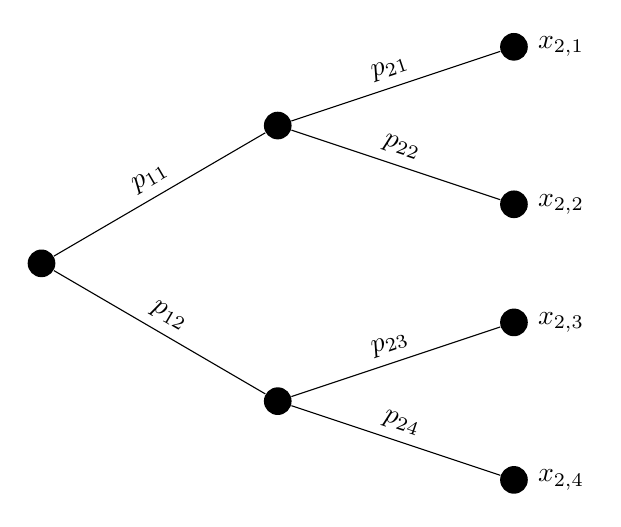
\begin{tikzpicture}[grow=right, sloped]
    \node[n1] {}
    child {
      node[n1] {}
      child {
        node[n1, label=right:
        {$x_{2,4}$}] {}
        edge from parent
        node[above] {$p_{24}$}
      }
      child {
        node[n1, label=right:
        {$x_{2,3}$ }] {}
        edge from parent
        node[above] {$p_{23}$}
      }
      edge from parent
      node[above] {$p_{12}$}
    }
    child {
      node[n1] {}
      child {
        node[n1, label=right:
        {$x_{2,2}$ }] {}
        edge from parent
        node[above] {$p_{22}$}
      }
      child {
        node[n1, label=right:
        {$x_{2,1}$ }] {}
        edge from parent
        node[above]  {$p_{21}$}
      }
      edge from parent
      node[above] {$p_{11}$}
    };
  \end{tikzpicture}


\end{frame}


%%%%%%%%%%%%%
%######################################
% Inicio comentario

%%%

\begin{frame}{Scenario trees}

\begin{itemize}
\item Assume that the stochastic process $\xi=(\xi_1,\ldots,\xi_T)$ has a finite number $K$ of realizations

\item Each realization (sequence) is called a scenario $\xi^i=(\xi_1^i,\ldots,\xi_T^i)$

\item Each scenario $\xi^i=(\xi_1^i,\ldots,\xi_T^i)$ has a probability $p_i>0$ associated

\item The value of a given scenario $\xi^i$ at stage $t$ is
denoted a node of the tree
\item The set of all nodes at stage $t$ is denoted by $\Omega_t$
%\item $\Omega_1$ contains only the \emph{root node}
\item The total number of scenarios is $K= |\Omega_T|$
\item We sometimes use the short hand $\iota$ to denote a node: $\iota \in
\Omega_t$
%\item Each scenario $\xi^i$ has a unique node at stage $t=1,2,\ldots,T$

\item The ancestor of a node $\iota \in \Omega_t$ is $a(\iota) \in\Omega_{t-1}$
%(the root node does have a ancestor)

\item The set of descendants (children) of a node $\iota \in \Omega_t$ is denoted by $C_\iota$
\item $\Omega_{t+1} = \cup_{\iota \in \Omega_t} C_\iota$, and $C_\iota \cap C_{\iota '} =\emptyset$ if $\iota \neq\iota '$
%\item Nodes in $\Omega_T$ does have children. Such nodes are called leave nodes.
\item $\mathcal{S}^{(\iota)}$ is the set of all scenarios passing through node $\iota$

\item The probability of node $\iota$ is $p^{(\iota)}:=\prob[\mathcal{S}^{(\iota)}]$

\item Conditional probability $\rho_{a\iota} = \frac{p^{(\iota)}}{p^{(a)}}$ if $a = a(\iota)$
\item  The probability of reaching a node $\iota\in \Omega_t$ is $p^{(\iota)}=\rho_{\iota_1\iota_2}\rho_{\iota_2\iota_1}\ldots \rho_{\iota_{t-1}\iota_t} = \prob[\mathcal{S}^{(\iota)}]$
\end{itemize}
\end{frame}
%#######################################################
%%%

\begin{frame}{Nested formulation}
\begin{block}{Linear case}
{\scriptsize
\[
\min_{\underset{x_1\ge 0}{A_1x_1=b_1}} c_1^\top  x_1+ \E\left[ \min_{\underset{x_2\ge 0}{B_2x_1 + A_2x_2=b_2}}c_2^\top x_2 + \E \left[\cdots+\E   [ \min_{\underset{x_T\ge 0}{B_Tx_{T-1} + A_Tx_T=b_T}}c_T^\top  x_T ]\right]\right]
\]
}
\end{block}
\begin{block}{Linear case + scenario tree}
{\tiny
\if{
\[
\!\!\!\!\!\!\!\!\!\!\!\!\!\!\!\!\!\!\!\!\!\!
%\min_{\underset{x_1\ge 0}{A_1x_1=b_1}} c_1^\top  x_1+ \sum_{\iota_2 \in \Omega_2}p^{\iota_2}\left[ \min_{\underset{x_2\ge 0}{B_2x_1 + A_2x_2=b_2}}c_2^\top x_2 + \sum_{\iota_3 \in \Omega_3}p^{(\iota_3)} \left[\cdots+\sum_{\iota_T \in \Omega_T} p^{(\iota_T)}  [ \min_{\underset{x_T\ge 0}{B_Tx_{T-1} + A_Tx_T=b_T}}c_T^\top  x_T ]\right]\right]
\min_{\underset{x_1\ge 0}{A_1x_1=b_1}} c_1^\top  x_1+ \sum_{\iota_2 \in \Omega_2}\rho_{1\iota_2}\left[ \min_{\underset{x_2\ge 0}{B_2x_1 + A_2x_2=b_2}}c_2^\top x_2 + \sum_{\iota_3 \in \Omega_3}\rho_{\iota_2\iota_3} \left[\cdots+\sum_{\iota_T \in \Omega} \rho_{\iota_{T-1}\iota_T}  [ \min_{\underset{x_T\ge 0}{B_Tx_{T-1} + A_Tx_T=b_T}}c_T^\top  x_T ]\right]\right]
\]
%
%\pause
%\azul{Ops! I forgot to name the nodes...}
}\fi
\[
\begin{array}{l}
\displaystyle\min_{\underset{x_1\ge 0}{A_1x_1=b_1}} c_1^\top  x_1+ \displaystyle \sum_{\iota_2 \in \Omega_2}\rho_{1\iota_2}\left[ \displaystyle \min_{\underset{x_2\ge 0}{B_2^{\iota_2}x_1 + A_2^{\iota_2}x_2=b_2^{\iota_2}}}{c_2^{\iota_2}}^\top x_2 + \displaystyle\sum_{\iota_3 \in \Omega_3}\rho_{\iota_2\iota_3} \Biggl[\cdots+\right.  \\
%
\quad \quad \quad \ldots +\left. \left.\displaystyle\sum_{\iota_T \in \Omega} \rho_{\iota_{T-1}\iota_T}  \left[ \displaystyle\min_{\underset{x_T\ge 0}{B_T^{\iota_T}x_{T-1} + A_T^{\iota_T}x_T=b_T^{\iota_T}}}{c_T^{\iota_T}}^\top  x_T \right]\right]\right]
\end{array}
\]
}
\end{block}
\end{frame}

%
\begin{frame}{Equivalent deterministic}
Denoting $\xi_t^{\iota_i} = (c_t^{\iota_i},B_t^{\iota_i},A_t^{\iota_i},b_t^{\iota_i})$ we can rewrite the above problem as

{\tiny
\[
\!\!\!\!\!\!\!\!\!\!\!\!\!\!\!\!\!\!\!\!\!\!
\left\{
\begin{array}{llllllll}
 \min & \displaystyle c_1^\top  x_1 &+& \sum_{\iota_2 \in \Omega_2}p^{(\iota_2)} {c_2^{\iota_2}}^\top x_2^{\iota_2} &+& \sum_{\iota_3 \in \Omega_3}p^{(\iota_3)} {c_3^{\iota_3}}^\top x_3^{\iota_3} &+ \cdots+&\sum_{\iota_T \in \Omega} p^{(\iota_T)}  {c_T^{\iota_T}}^\top  x_T^{\iota_T} \\
\mbox{s.t.} & A_1x_1 &&&&&&=b_1\\
&B_2^{\iota_2} x_1 &+& A_2^{\iota_2}x_2^{\iota_2}  &&&&= b_2^{\iota_2}  \; \forall \iota_2 \in \Omega_2\\
%
&&&B_3^{\iota_3} x_2^{a(\iota_3)} &+& A_3^{\iota_3}x_3^{\iota_3}  &&= b_3^{\iota_3}  \; \forall \iota_3 \in \Omega_3\\
&&& \ddots && \ddots\\
&&&B_T^{\iota_T} x_{T-1}^{a(\iota_T)} &+& A_T^{\iota_T}x_T^{\iota_T}  &&= b_T^{\iota_T}  \; \forall \iota_T \in \Omega_T
\end{array}
\right.
\]
}
\azul{This is a LP!}
\pause

Example:
\begin{itemize}
\item Suppose $T=12$, each node $\iota_t \in \Omega_t$ has 4 children
\end{itemize}
This gives $4^{11} = 4,194,304$ scenarios.
\begin{itemize}
\item Suppose each $x_t \in \Re^{100}$, $t=1,\ldots,12$
\end{itemize}
\pula
\verm{The number of variables of the above problem is approximately $4.59\times 10^8$!}
\end{frame}

\begin{frame}{Dynamic programming formulation}
\begin{itemize}
\item Stage $t=T$
\[
Q_T(x_{T-1},\xi_{[T]}^\iota):= \min_{\underset{x_T\ge 0}{B_T^\iota x_{T-1}^{a(\iota)} + A_T^\iota x_T=b_T^\iota}}{c_T^\iota}^\top  x_T
\]
\pula
\pause
\item At stages $t=2,\ldots,T-1$
\[
Q_t(x_{t-1},\xi_{[t]}^\iota):= \min_{\underset{x_t\ge 0}{B_t^\iota x_{t-1}^{a(\iota)} + A_t^\iota x_t=b_t^\iota }} {c_t^\iota}^\top  x_t +
\sum_{j \in C_\iota} p^{(j)}\left[Q_{t+1}(x_t,\xi_{[t+1]}^j)\right]
\]
\pula
\pause
\item Stage $t=1$
\verm{
\[
\min_{\underset{x_1\geq 0}{A_1x_1=b_1}} c_1^\top x_1 + \sum_{\iota \in C_1}p^{(\iota)}\left[Q_2(x_1,\xi_2^\iota)\right]
\]
}
\end{itemize}
\end{frame}


\begin{frame}{Dynamic programming formulation}
\begin{itemize}
\item Stage $t=T$
\[
Q_T(x_{T-1},\xi_{[T]}^\iota):= \min_{\underset{x_T\ge 0}{B_T^\iota x_{T-1}^{a(\iota)} + A_T^\iota x_T=b_T^\iota}}{c_T^\iota}^\top  x_T
\]
\pula

\item At stages $t=2,\ldots,T-1$
\[
\underline{Q_t}(x_{t-1},\xi_{[t]}^\iota):= \min_{\underset{x_t\ge 0}{B_t^\iota x_{t-1}^{a(\iota)} + A_t^\iota x_t=b_t^\iota }} {c_t^\iota}^\top  x_t +
\sum_{j \in C_\iota} p^{(j)}\left[\underline{ Q_{t+1}}(x_t,\xi_{[t+1]}^j)\right]
\]
\pula
\item Stage $t=1$
\verm{
\[
\min_{\underset{x_1\geq 0}{A_1x_1=b_1}} c_1^\top x_1 + \sum_{\iota \in C_1}p^{(\iota)}\left[\underline{ Q_2}(x_1,\xi_2^\iota)\right]
\]
}
\end{itemize}
\end{frame}


\begin{frame}{Dynamic programming formulation}
\begin{itemize}
\item Stage $t=T$
\[
Q_T(x_{T-1},\xi_{[T]}^\iota):= \min_{\underset{x_T\ge 0}{B_T^\iota x_{T-1}^{a(\iota)} + A_T^\iota x_T=b_T^\iota}}{c_T^\iota}^\top  x_T
\]
\pula

\item At stages $t=2,\ldots,T-1$
\[
\underline{Q_t}(x_{t-1},\xi_{[t]}^\iota):= \min_{\underset{x_t\ge 0}{B_t^\iota x_{t-1}^{a(\iota)} + A_t^\iota x_t=b_t^\iota }} {c_t^\iota}^\top  x_t +\check{\Q}_{t+1}(x_t,\xi_{[t]}^{\iota})
\]
%
\[
\check{\Q}_{t+1}(x_{t},\xi_{[t]}^\iota):= \sum_{j \in C_{\iota}}p^{(j)}\left[\underline{Q_{t+1}}(x_{t},\xi_{[t+1]}^j)\right]
\]
\pula
\item Stage $t=1$
\verm{
\[
\min_{\underset{x_1\geq 0}{A_1x_1=b_1}} c_1^\top x_1 + \check{\Q}_{2}(x_2,\xi_{[1]})
\]
}
\end{itemize}
\azul{Cutting-plane approximation}
\end{frame}
%%%%%%%%%%%%%%%%
\begin{frame}{Assumptions}
\begin{itemize}
\item The set of nodes $\Omega_t$ has finitely many elements
\pula
\item the problem has relatively complete recourse

\end{itemize}
\pula
\azul{The last hypotheses is made only for sake of simplicity!}
\end{frame}
%%%%
\begin{frame}{Cutting-plane approximation}
\begin{itemize}
\item Stage $t=T$
\[
Q_T(x_{T-1}^k,\xi_{[T]}):= \min_{\underset{x_T\ge 0}{B_T x_{T-1}^{k} + A_T x_T=b_T}}{c_T}^\top  x_T
\]
\pula

\item At stages $t=2,\ldots,T-1$
\[
\azul{\underline{Q_t}(x_{t-1}^k,\xi_{[t]})}:=
\left\{ \begin{array}{llll}
\displaystyle\min_{x_t\geq 0,r_{t+1}} & {c_t}^\top  x_t +r_{t+1} \\
\mbox{s.t.} & B_t x_{t-1}^{k} + A_t x_t=b_t  \\
            & r_{t+1} \geq \alpha_{t+1}^j + \beta_{t+1}^j x_t & j=1,\ldots,k
\end{array}\right.
\]
\pula
\item Stage $t=1$
\[
\verm{\underline{z}^k}:=\left\{ \begin{array}{lll}
\displaystyle \min_{x_1\geq 0,r_2} &  c_1^\top x_1 + r_2\\
\mbox{s.t.} & A_1x_1=b_1 \\
           & r_{2} \geq \alpha_{2}^j + \beta_{2}^j x_1 & j=1,\ldots,k
\end{array}
\right.
\]

\end{itemize}
\end{frame}
%%%%%%%%%%%
\begin{frame}{Cutting-plane approximation}
\begin{itemize}
\item At stages $t=2,\ldots,T-1$
\[
\azul{\underline{Q_t}(x_{t-1}^k,\xi_{[t]})}:=
\left\{ \begin{array}{llll}
\displaystyle\min_{x_t\geq 0,r_{t+1}} & {c_t}^\top  x_t +r_{t+1} \\
\mbox{s.t.} & B_t x_{t-1}^{k} + A_t x_t=b_t  &&\verm{(\pi_t)}\\
            & r_{t+1} \geq \alpha_{t+1}^j + \beta_{t+1}^j x_t & j=1,\ldots,k & \verm{(\rho_j)}
\end{array}\right.
\]

\pula
\item Cuts ($t=T$)
\[
\alpha_T^k := \E_{|\xi_{T-1}}[b_T^\top \pi_T^k]\quad \mbox{and}\quad
\beta_T^k: =  -\E_{|\xi_{T-1}}[B_T^\top \pi_T^k]
\]
\pula
\item Cuts ($t=T-1,\ldots, 2$)
\[
\alpha_t^k := \E_{|\xi_{t-1}}[b_t^\top \pi_t^k + \sum_{j=1}^k \alpha_{t+1}^j \rho_k^j]\quad \mbox{and}\quad
\beta_t^k: =  -\E_{|\xi_{t-1}}[B_t^\top \pi_t^k]
\]
\end{itemize}
\end{frame}

%%%%
\begin{frame}{Nested decomposition - (nested L-shaped method)}
\begin{itemize}
\item  J.R. Birge (1985)
\end{itemize}
\begin{block}{It has two main steps:}
\begin{itemize}
\item \alert{Forward} that goes from $t=1$ up to $t=T$ solving subproblems to define policy $x_t^k(\xi_t)$
\begin{itemize}
\item In this step an upper bound $\overline{z}^k$ for the optimal value is determined
\end{itemize}

\pula
\item \alert{Backward} that comes from $t=T$ up to $t=1$ solving subproblems to compute linearizations that improve the cutting-plane approximation.

\begin{itemize}
\item In this step a lower bound $\underline{z}^k$ is obtained
\end{itemize}
\end{itemize}
\end{block}
\begin{block}{Stopping test}
\begin{itemize}
\item The Nested decomposition stops when
\[\overline{z}^k-\underline{z}^k \le \texttt{Tol}.\]
\item In this case $x_1^k$ is a $\texttt{Tol}$-solution to the T-SLP
\end{itemize}
\end{block}
\end{frame}
%%
%%
\begin{frame}{Forward and Backward steps}
\begin{center}
\includegraphics[width=7cm]{../Figs/EtapasProgRegr.pdf} {}
\end{center}
%{ \centerline{\includegraphics[width=7.5cm]{EtapasProgRegr.pdf}}}
\end{frame}
%%
\begin{frame}{Algorithm - Nested decomposition}
{stages $t=2,\ldots,T-1$
\[
\azul{\underline{Q_t}(x_{t-1}^k,\xi_{[t]})}:=
\left\{ \begin{array}{llll}
\displaystyle\min_{x_t\geq 0,r_{t+1}} & {c_t}^\top  x_t +r_{t+1} \\
\mbox{s.t.} & B_t x_{t-1}^{k} + A_t x_t=b_t  &&\verm{(\pi_t)}\\
            & r_{t+1} \geq \alpha_{t+1}^j + \beta_{t+1}^j x_t & j=1,\ldots,k & \verm{(\rho_j)}
\end{array}\right.
\]
}
{\scriptsize
\begin{itemize}
\item {\bf Step 0: inicialization}. Define $k=1$ and add the constraint $r_t = 0$ in all LPs $\underline{Q_t}$, $t=2,\ldots,T-1$
Compute $\underline{z}^1$ and let its solution be $x_1^{1}$
\pula
\item {\bf Step 1: forward}.
For t=2,\ldots,T, solve the LP $\underline{Q_t}$ to obtain $x_t^k:=x_t^k(\xi_{[t]})$. Define $\bar z^k := \E[\sum_{t=1}^T c_t^\top x_t^k]$
\pula
\item {\bf Step 2: backward}. Compute $\alpha_T^k$ and $\beta_T^k$.
Set $t=T$. Loop:
\begin{itemize}
\item While $t>2$
\item $t\gets t-1$
\item solve the LP $\underline{Q_t}(x_{t-1}^k,\xi_{[t]})$
\item Compute  $\alpha_t^k$ and $\beta_t^k$
\end{itemize}

Compute $\underline{z}^k$ and let its solution be $x_1^{k+1}$
\pula
\item {\bf Step 3: Stopping test}.  If $\bar z^k - \underline{z}^k\leq \epsilon$, stop. Otherwise set $k\gets k+1$ and \\ go back to Step 1
\end{itemize}
}
\end{frame}


%%%%%%%%%%%%%%%%%%%%%%%%%%%%%%%%%%%%
\begin{frame}{Nested decomposition - iterative process}
\begin{center}
\includegraphics[width=11cm]{../Figs/v1} {}
\end{center}
\begin{itemize}
\item $\min_{\underset{x_1\geq 0}{A_1x_1=b_1}} c_1^\top x_1 + \alert{\Q}_{2}(x_2,\xi_{[1]})$
\pula
\item $
\alert{\Q}_{t+1}(x_t,\xi_{[t]})=\E_{|\xi_{[t]}}[\verde{Q}_{t+1}(x_t,\xi_{[t+1]})]\; \mbox{ for }\; t=1,\ldots,T-1\,,
$
and  $\Q_{T+1}(x_T,\xi_{[T]}) =0$
\pula
%A fun��o de recurso m�dio $\Q$ usa as fun��es de recurso
\item $
\verde{Q}_{t}(x_{t-1},\xi_{[t]})=\min \; c_{t}^\top x_{t} +  \alert{\Q}_{t+1}(x_{t},\xi_{[t]})\;\mbox{ s.t. }\;\underset{x_{t}\geq 0}{B_{t}x_{t-1}+A_{t}x_{t}=b_{t}}
$
\end{itemize}
\end{frame}
%
\begin{frame}{Nested decomposition - iterative process}
\begin{center}
\includegraphics[width=11cm]{../Figs/v2} {}
\end{center}
\begin{itemize}
\item $\min_{\underset{x_1\geq 0}{A_1x_1=b_1}} c_1^\top x_1 + \azul{\check{\Q}}_{2}(x_2,\xi_{[1]})$
\pula
\item $
\azul{\check{\Q}}_{t+1}(x_t,\xi_{[t]})=\E_{|\xi_{[t]}}[\underline{{Q}_{t+1}}(x_t,\xi_{[t+1]})]\; \mbox{ for }\; t=1,\ldots,T-1\,,
$
e  $\check{\Q}_{T+1}(x_T,\xi_{[T]}) =0$
\pula
%A fun��o de recurso m�dio $\Q$ usa as fun��es de recurso
\item $
\underline{Q_{t}}(x_{t-1},\xi_{[t]})=\min \; c_{t}^\top x_{t} +  \azul{\Q}_{t+1}(x_{t},\xi_{[t]})\;\mbox{ s.t. }\;\underset{x_{t}\geq 0}{B_{t}x_{t-1}+A_{t}x_{t}=b_{t}}
$

\item \azul{Figures by Vincent Guigues}

\end{itemize}

\end{frame}
%
\begin{frame}{Nested decomposition - iterative process}
\begin{center}
\includegraphics[width=11cm]{../Figs/v3} {}
\doublebox{Forward step}
\end{center}

\end{frame}
%
\begin{frame}{Nested decomposition - iterative process}
\begin{center}
\includegraphics[width=11cm]{../Figs/v4} {}
\doublebox{Backward step}
\end{center}
\end{frame}
%
\begin{frame}{Nested decomposition - iterative process}
\begin{center}
\includegraphics[width=11cm]{../Figs/v5} {}
\doublebox{Backward step}
\end{center}
\end{frame}
%
\begin{frame}{Nested decomposition - iterative process}
\begin{center}
\includegraphics[width=11cm]{../Figs/v6} {}
\doublebox{Backward step}
\end{center}
\end{frame}
%
\begin{frame}{Nested decomposition - iterative process}
\begin{center}
\includegraphics[width=11cm]{../Figs/v7} {}
\doublebox{Backward step}
\end{center}
\end{frame}
%
\begin{frame}{Nested decomposition - iterative process}
\begin{center}
\includegraphics[width=11cm]{../Figs/v8} {}
\doublebox{Forward step}
\end{center}
\end{frame}
%
\begin{frame}{Nested decomposition - iterative process}
\begin{center}
\includegraphics[width=11cm]{../Figs/v9} {}
\doublebox{Forward step}
\end{center}
\end{frame}
%
\begin{frame}{Nested decomposition - iterative process}
\begin{center}
\includegraphics[width=11cm]{../Figs/v10} {}
\doublebox{Forward step}
\end{center}
\end{frame}
%
\begin{frame}{Nested decomposition - iterative process}
\begin{center}
\includegraphics[width=11cm]{../Figs/v11} {}
\doublebox{Forward step}
\end{center}
\end{frame}
%
\begin{frame}{Nested decomposition - iterative process}
\begin{center}
\includegraphics[width=11cm]{../Figs/v12} {}
\doublebox{Backward step}
\end{center}
\end{frame}
%
\begin{frame}{Nested decomposition - iterative process}
\begin{center}
\includegraphics[width=11cm]{../Figs/v13} {}
\doublebox{Backward step}
\end{center}
\end{frame}
%
\begin{frame}{Nested decomposition - iterative process}
\begin{center}
\includegraphics[width=11cm]{../Figs/v14} {}
\doublebox{Backward step}
\end{center}
\end{frame}
%
\begin{frame}{Nested decomposition - iterative process}
\begin{center}
\includegraphics[width=11cm]{../Figs/v15} {}
\doublebox{Backward step}
\end{center}
\end{frame}
%
\begin{frame}{Nested decomposition - iterative process}
\begin{center}
\includegraphics[width=11cm]{../Figs/v16} {}
\doublebox{Forward step}
\end{center}
\end{frame}
%
\begin{frame}{Nested decomposition - iterative process}
\begin{center}
\includegraphics[width=11cm]{../Figs/v17} {}
\doublebox{Forward step}
\end{center}
\end{frame}
%
\begin{frame}{Nested decomposition - iterative process}
\begin{center}
\includegraphics[width=11cm]{../Figs/v18} {}
\doublebox{Forward step}
\end{center}
\end{frame}
%
\begin{frame}{Nested decomposition - iterative process}
\begin{center}
\includegraphics[width=11cm]{../Figs/v19} {}
\doublebox{Forward step}
\end{center}
\end{frame}
%
\begin{frame}{Nested decomposition - iterative process}
\begin{center}
\includegraphics[width=11cm]{../Figs/v20} {}
\doublebox{Backward step}
\end{center}
\end{frame}
%
\begin{frame}{Nested decomposition - iterative process}
\begin{center}
\includegraphics[width=11cm]{../Figs/v21} {}
\doublebox{Backward step}
\end{center}
\end{frame}
%
\begin{frame}{Nested decomposition - iterative process}
\begin{center}
\includegraphics[width=11cm]{../Figs/v22} {}
\doublebox{Backward step}
\end{center}
\end{frame}
%
\begin{frame}{Nested decomposition - iterative process}
\begin{center}
\includegraphics[width=11cm]{../Figs/v23} {}
\doublebox{Backward step}
\end{center}
\begin{itemize}
\item Figures by Vincent Guigues.
\end{itemize}
\end{frame}

\begin{frame}{Convergence analysis}

\begin{block}{Assumptions}
\begin{itemize}
\item The set of nodes $\Omega_t$ has finitely many elements, $t=1,\ldots,T$
\pula
\item the problem has recourse relatively complete \azul{(for simplicity, only)}
\pula
\item the feasible set, in each stage $t=1,\ldots,T$, is compact

\end{itemize}
\end{block}
\pula
\begin{lemma}
$
\check \Q^k_t(x_{t-1},\xi_{[t-1]}) \leq  \Q_t(x_{t-1},\xi_{[t-1]}) \quad \forall\; x_{t-1} \; \mbox{ and }\; \forall t=2,\ldots,T
$
\end{lemma}
\pula

\begin{theorem}
The Nested Decomposition converges finitely to an optimal solution of the considered T-SLP
\end{theorem}
\end{frame}

\begin{frame}{Scenario tree}
  \tikzstyle{level 1}=[level distance=3cm, sibling distance=3.5cm]
  \tikzstyle{level 2}=[level distance=3cm, sibling distance=2cm]
  \tikzstyle{level 3}=[level distance=3cm, sibling distance=1cm]
  % Define styles for bags and leafs
  \tikzstyle{n1} = [circle, minimum width=10pt,fill, inner sep=0pt]

  % The sloped option gives rotated edge labels. Personally
  % I find sloped labels a bit difficult to read. Remove the sloped options
  % to get horizontal labels.
  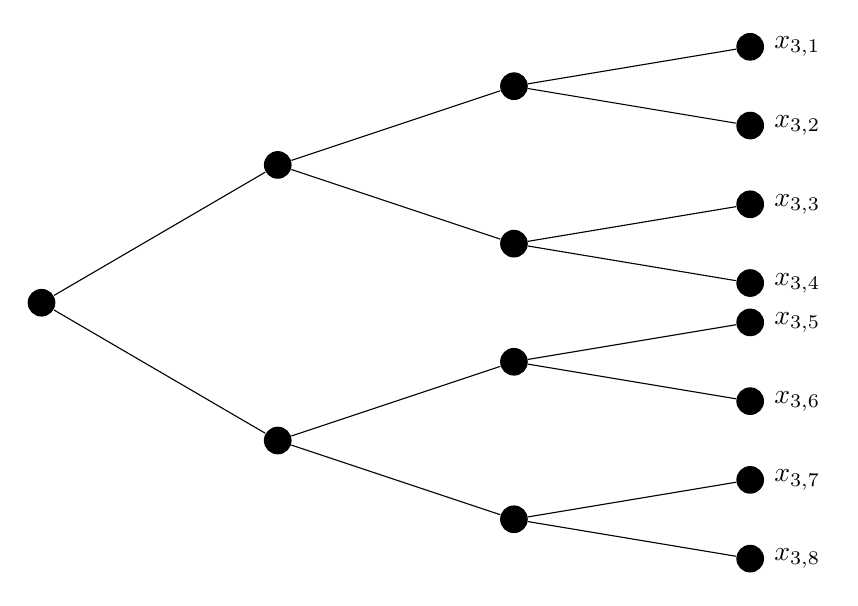
\begin{tikzpicture}[grow=right, sloped]
    \node[n1] {}
    child {
      node[n1] {}
      child {
        node[n1, label=right:
        {}] {}
        child {
          node[n1, label=right:
          {$x_{3,8}$}] {}
          edge from parent
        }
        child {
          node[n1, label=right:
          {$x_{3,7}$}] {}
          edge from parent
        }
        edge from parent
      }
      child {
        node[n1, label=right:
        {}] {}
        child {
          node[n1, label=right:
          {$x_{3,6}$}] {}
          edge from parent
        }
        child {
          node[n1, label=right:
          {$x_{3,5}$}] {}
          edge from parent
        }
        edge from parent
      }
      edge from parent
    }
    child {
      node[n1] {}
      child {
        node[n1, label=right:
        {}] {}
        child {
          node[n1, label=right:
          {$x_{3,4}$}] {}
          edge from parent
        }
        child {
          node[n1, label=right:
          {$x_{3,3}$}] {}
          edge from parent
        }
        edge from parent
      }
      child {
        node[n1, label=right:
        {}] {}
        child {
          node[n1, label=right:
          {$x_{3,2}$}] {}
          edge from parent
        }
        child {
          node[n1, label=right:
          {$x_{3,1}$}] {}
          edge from parent
        }
        edge from parent
      }
      edge from parent
    };
  \end{tikzpicture}


  \begin{block}{Question}
    Can we compress the information?
  \end{block}

\end{frame}

\begin{frame}{Information structure}
  In multistage problems, decisions are sequential in nature
  \begin{equation*}
    x_0 \leadsto \xi_1 \leadsto x_1 \leadsto \xi_2 \leadsto \cdots \leadsto x_T
  \end{equation*}
  The sequence $\{\xi_t\}$ is a \emph{stochastic process}.

  \begin{block}{Non-anticipativity}
    We note $\xi_{[t]} := \{\xi_1, \cdots, \xi_{t-1}\}$ the information
    available up to time $t$.  \\
    The process $\{x_t\}_t$ is \emph{non-anticipative} if
    for all $t$, the values of $x_t$ depends only on the past information:
    \begin{equation*}
      x_t = x_t(\xi_{[t]}) \; .
    \end{equation*}
  \end{block}
\end{frame}


\begin{frame}{Information structure \#1: Stage-wise independence}
  \begin{block}{Stage-wise independence}
    Assume uncertainties $\xi_1, \cdots, \xi_T$ are time-step independent: \\
    for all $t$, the random variable $\xi_t$ is stochastically independent from $\xi_{[t-1]}$.
  \end{block}

  \vspace{2cm}

  \tikzstyle{n1} = [circle, minimum width=10pt,fill, inner sep=0pt]

  % The sloped option gives rotated edge labels. Personally
  % I find sloped labels a bit difficult to read. Remove the sloped options
  % to get horizontal labels.
  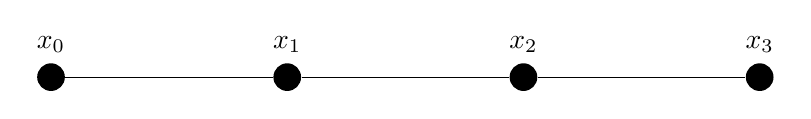
\begin{tikzpicture}[grow=right, sloped]
    \node[n1, label=above:{$x_0$}] (N1) at (0, 0) {};
    \node[n1, label=above:{$x_1$}] (N2) at (3, 0) {};
    \node[n1, label=above:{$x_2$}] (N3) at (6, 0) {};
    \node[n1, label=above:{$x_3$}] (N4) at (9, 0) {};
    \draw (N1) -- (N2);
    \draw (N2) -- (N3);
    \draw (N3) -- (N4);
  \end{tikzpicture}

  \vspace{2cm}

  The tree reduces to a line: \\ we will prove that $x_4$ depends only on the values in $x_3$,
  not on $x_2, x_1$

\end{frame}



%%%%%
\begin{frame}{Dynamic programming formulation}
  \begin{block}{Proposition}
    Under stage-wise independence, the value functions $\{Q_t(\cdot, \xi)\}$
    satisfy \\ the Dynamic Programming backward recursions:
    setting $V_{T+1}(x_{T}) := 0$, we have for $t=T, \cdots, 1$,
    \begin{equation*}
      \left\{
      \begin{aligned}
      & Q_t(x_{t-1}, \xi) = \min_{x_t \geq 0 } \big[ c_t(\xi)^\top x_t + V_{t+1}(x_{t}) \big] \quad \text{s.t.} \quad B_t(\xi) x_{t-1} + A_t(\xi) x_t = b_t(\xi) \\
      & V_t(x_{t-1}) = \mathbb{E}_{\xi} \big[ Q_t(x_{t-1}, \xi) \big]
      \end{aligned}
      \right.
    \end{equation*}
  \end{block}

  \begin{block}{Theorem}
    A feasible policy $\{\overline{x}_t \}_t$ is \emph{optimal}
    if and only if, for all $t=1, \cdots, T$,
    \begin{equation*}
      \overline{x}_t(\xi_{[t]}) \in \argmin_{x_t \geq 0 } \; c_t(\xi_t)^\top x_t + V_{t+1}(x_t) \quad \text{s.t.} \quad B_t(\xi_t) x_{t-1} + A_t(\xi_t) x_t = b_t(\xi_t)
    \end{equation*}
    A direct corollary is that $\overline{x}_t(\xi_{[t]})$ depends only
    on the values of $x_{t-1}$ and of $\xi_t$.
  \end{block}

\end{frame}

%%%%
\begin{frame}{Optimality conditions: sensitivity propagate backward}

\begin{itemize}
\item Let the extended real-valued function $f_t(x_t,\xi) = \left\{\begin{aligned}
    c_t(\xi)^\top x_t & \quad \text{if } \quad x_t \geq 0  \\
    +\infty & \quad \text{otherwise}
\end{aligned}\right.$
\item Let the Lagrangian
  \begin{equation*}
    L(x_t, \pi_t) := f_t(x_t, \xi) + V_{t+1}(x_t) + \pi_t (b_t - B_t x_{t-1} - A_t x_t)
  \end{equation*}

% \pula
% \item $\bar \pi _t(\xi_{[t]}) \in \D(\bar x_{t-1}(\xi_{[t-1]}),\xi_{[t]})$
% \pula
% \item $\D(\bar x_{t-1}(\xi_{[t-1]}),\xi_{[t]})$ is the set of Lagrange multipliers of
% \[Q_t(x_{t-1},\xi_{[t]}):= \min_{\underset{x_t\ge 0}{B_tx_{t-1} + A_tx_t=b_t}} c_t^\top x_t +
% \Q_{t+1}(x_t,\xi_{[t]})\]
\end{itemize}

\begin{theorem}
Under some assumptions (e.g. finitely many scenarios and polyhedral $f_t$).
A feasible policy $\bar x_t(\xi_{[t]})$ is optimal iff there exists measurable $\bar \pi_t(\xi_{[t]})$, $t=1,\ldots,T$, such that
\[
  \verm{0\in \partial f_t(\bar x_t(\xi_{[t]}),\xi_t)  + \partial V_{t+1}(\bar x_t(\xi_{[t]})) - A_t^\top \bar \pi_t(\xi_{[t]})}
% - \E_{|\xi_{[t]}}[B_{t+1}^\top \bar \pi_{t+1}(\xi_{[t+1]})
\]
and
\begin{equation*}
  \verm{ \partial V_t(x_{t-1}) = \mathbb{E}_\xi \big[ - B_t^\top \bar \pi_t(\xi_{[t]}) \big]}
\end{equation*}
 for a.e. $\xi_{[t]}$ and $t=1,\ldots,T$
\end{theorem}
\end{frame}

\begin{frame}{Solution algorithm by discretization}
\RestyleAlgo{ruled}
  \begin{algorithm}[H]
    \caption{Stochastic Dynamic Programming (SDP)}
    \KwData{Set $V_{T+1} = 0$}
    Find a discretization $\mathbb{X}_d$ of feasible space $\mathcal{X}$;

    \For{$t=T, \cdots, 1$}{
      \For{$x_{t-1} \in \mathbb{X}_d$}{
        \For{$\xi_t \in \{\xi_t^1, \cdots, \xi_t^N \}$}{
          Solve $Q_t(x_{t-1}, \xi_t)$ using linear programming;
        }
        Set $V_{t}(x_{t-1}) = \sum_{i=1}^N p_i Q_t(x_{t-1}, \xi_t^i)$;
      }
    }
  \end{algorithm}

  \begin{block}{Complexity}
    Algorithm SDP solves a total number of (small) LP:
    \begin{equation*}
      \mathcal{O}(|\mathbb{X}_d| \times N \times T)
    \end{equation*}
  \end{block}
  Algorithm is useful only if dimension of the state is small
  (\emph{curse of dimensionality})
\end{frame}


%%%%

\begin{frame}{Information structure \#2: Markov chain}
  \begin{block}{Markov-chain lattice}
    The process $\{\xi_t\}_t$ is Markovian if for all $t$, the conditional
    distribution of $\xi_t$ given $\xi_{[t-1]}$ depends only on $\xi_{t-1}$.
  \end{block}

  \vspace{2cm}

  \tikzstyle{n1} = [circle, minimum width=10pt,fill, inner sep=0pt]

  % The sloped option gives rotated edge labels. Personally
  % I find sloped labels a bit difficult to read. Remove the sloped options
  % to get horizontal labels.
  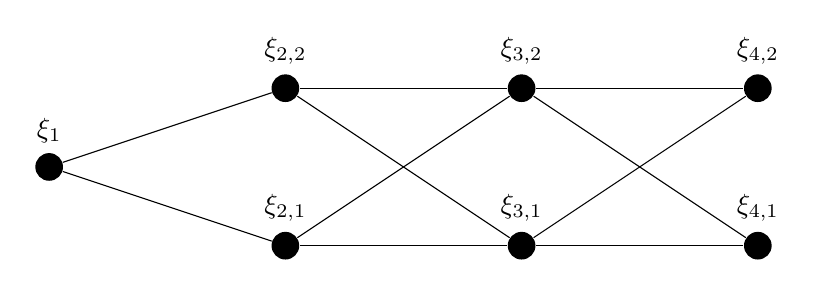
\begin{tikzpicture}[grow=right, sloped]
    \node[n1, label=above:{$\xi_1$}] (N1) at (0, 1) {};
    \node[n1, label=above:{$\xi_{2,1}$}] (N21) at (3, 0) {};
    \node[n1, label=above:{$\xi_{2,2}$}] (N22) at (3, 2) {};
    \node[n1, label=above:{$\xi_{3,1}$}] (N31) at (6, 0) {};
    \node[n1, label=above:{$\xi_{3,2}$}] (N32) at (6, 2) {};
    \node[n1, label=above:{$\xi_{4,1}$}] (N41) at (9, 0) {};
    \node[n1, label=above:{$\xi_{4,2}$}] (N42) at (9, 2) {};
    \draw (N1) -- (N21);
    \draw (N1) -- (N22);
    \draw (N21) -- (N31);
    \draw (N21) -- (N32);
    \draw (N22) -- (N31);
    \draw (N22) -- (N32);
    \draw (N31) -- (N41);
    \draw (N31) -- (N42);
    \draw (N32) -- (N41);
    \draw (N32) -- (N42);
  \end{tikzpicture}

\end{frame}

